\documentclass[12pt,twoside,oneright,a4paper,chapter=TITLE,english,brazil]{unipampa}
\usepackage[utf8]{inputenc}                 % O Latex deve ser escrito em utf-8, pois utiliza o pacote abntex2
\usepackage[alf,abnt-emphasize=bf]{abntex2cite}               % Pacote para utilizar a citação da abnt (Nome,ANO)
\usepackage{times}                          % Usa a fonte padrao Times new roman
%\usepackage{pdfpages}                      % Usar quando for adicionar a folha de aprovação assinada
\usepackage{graphicx}                       % Usar para incluir figuras
\usepackage{float}                          % Permite travar as figuras usando o parametro [H]
\usepackage{makeidx}\makeindex              % Usar para criar indexação no texto


% Configuração do documento (autor, titulo, orientação ....)

% Autor, para varios autores use: \and entre eles
\autortrabalho{Garcia}{Patrick Rogger}           
\autor{Patrick Rogger Garcia}

% Titulo do trabalho
\titulo{Desenvolvimento de Software livre para processamentos de dados magnetotelúricos}                

% Orientador e Coorientador
\orientador[Orientador]{Vinicius Abreu de Oliveira}
\coorientador[Co-orientadora]{Andréa Cristina Lima dos Santos Matos}

% Curso
\curso{geofísica}                           

% LOCAL
\local{Caçapava do Sul}
\data{\the\year}            % Pode ser passado um ano especifico. Ex. \data{2018}

% Tipo do Trabalho
\tipotrabalho{Trabalho de Conclusão de Curso (Graduação)}

% Preambulo do Trabalho 
\preambulo{\imprimirtipotrabalho{} apresentado ao curso
            de Bacharelado em \imprimircurso{} da Universidade
            Federal do Pampa como requisito
            parcial para obtenção do grau de Bacharel em \imprimircurso.}

% Codigo cutter            
\cutter{G216d} % Se não tiver, deixe em branco

% Area de concentração
\areadeconcentracao{Geofísica Espacial, Geofísica de software}

% Texto da defesa
\defesa{Trabalho de Conclusão de Curso defendido e aprovado em: 11 de novembro de 2018.}

% Membros da Banca
% ======================================================================================
\titulacaoorientador{Prof. Post.}             % Titulação do orientador
\membroA{Prof. Dr.}{Éverton Frigo}{UNIPAMPA}  % Utilize o formato \membroA{Titulo}{NOME}{INSTITUIÇÃO}
\membroB{Titulo}{NOME}{INSTITUIÇÃO}           %
% ======================================================================================

% Palavras Chaves (Portugues): A-J
\chaveA{Magnetotelúrico}
\chaveB{Python3}
\chaveC{Software Livre}
%=================================

% Palavras Chaves (Ingles): A-J
\keywordA{Magnetotelluric}
\keywordB{Python3}
\keywordC{Free Software}
%=================================


% INICIO DO DOCUMENTOS
\begin{document}
\imprimircapa                   % Imprime a Capa

\imprimirfolhaderosto*          % Imprime a Folha de Rosto, 
                                % Para gerar o pdf sem a ficha Catalografica no verso, retire o '*'

\imprimirfichacatalografica     % Imprime a Ficha Catalografica

\imprimirfolhadeaprovacao       % Imprime a Folha de Aprovação
%\includepdf{folhadeaprovacao_digitalizada.pdf}    % Use para adicionar a versão digitalizada com as assinaturas


% DEDICATORIA 
% ===================================
\begin{dedicatoria}
    tectodsdfa dffds dddf
\end{dedicatoria}
% ===================================


% AGRADECIMENTOS
% ===================================
\begin{agradecimentos}
    Eu agradeco a um minhao de pessoa por tudoi que foi feito e como esta sendo utilizado a paltaforma para novos usuariso e mnomanetos de alegria e todo o mundo
    
    \noindent sfdsfsdg kjkas djfuwernwer sdgfsdddd
\end{agradecimentos}
% ===================================


% EPÍGRAFE
% ===================================
\begin{epigrafe}
    Moça boinita moça bem feita
    \DoubleSpacing \\
    -- (Sr. Madruga)
\end{epigrafe}
% ===================================


% RESUMO (PORTUGUES)
% ===================================
\begin{resumo}
 aqui fica o resumo
\end{resumo}
% ===================================


% RESUMO (INGLES)
% ===================================
\begin{resumoingles}
 This abstract
\end{resumoingles}
% ===================================


% LISTA DE FIGURAS E TABELAS
% ================================================
\listoffigures      % Imprime a lista de figuras
\listoftables       % Imprime a lista de tabelas
% ================================================


% LISTA DE SIGLAS E ABREVIATURAS
% ==============================================================
% Utilize o formato:
%   \item[SIGLA --]         Nome da sigla
\begin{siglas}
    \item[UNIPAMPA --]         Universidade Federal do Pampa
    \item[MT --]               Magnetotelúrico
\end{siglas}
% ==============================================================


% LISTA DE SÍMBOLOS
% ==============================================================
% Utilize o formato:
%   \item[Simbolo --]         Nome do símbolo
\begin{simbolos}
    \item[$ \nabla $ -- ]       Nabla
\end{simbolos}
% ==============================================================


% SUMÁRIO
% ==============================================================
\tableofcontents       % Imprime o sumario
% ==============================================================


% CORPO DO TEXTO
% =============================================================================
%
% Hierarquia:
% \chapter{NOME DO CAPITULO}                 --- secção primária   | 1.
%    \section{Nome da secção}                --- secção secundária | 1.1
%       \subsection{Nome da Secção primeria} --- secção terciária  | 1.1.1
%          \subsubsection{Nome}              --- secção quaternária| 1.1.1.1  
%              \subsubsubsection{Nome}       --- secção quinária   | 1.1.1.1.1
%
\textual                    % Inicia os elementos Textuais
\pagestyle{simple}          % Retira a linha e titulo no verso das paginas
\OnehalfSpacing             % Ajusta o texto para 1.5 entre linhas
% =============================================================================

\chapter{INTRODUÇÃO}
    
     O método geofísico \index{magnetotelúrico}, utiliza as baixas frequências do espectro eletromagnético, para investigar a subsuperfície do planeta Terra. A interação do vento solar com o campo magnético terrestre, compõe a origem dessas ondas eletromagnéticas.  
    
    A grande complexidade dos dados desestimula o desenvolvimento de para o processamento dos mesmos. Atualmente os programas destinados a esse tipo de atividade são proprietários,\cite{cagniard1953basic} com alto valor comercial, ou são livres operacionais exclusivamente por linhas de comando.  
    
    A comunidade MTnet, mantém laços com diversos pesquisados na área do MT, e reúne as aplicações destinadas aos processamentos, tais como:  de pré-processamento, inversão, tratamento estatísticos, dentre outros. Os programas alocados no MTnet são de uso livre e destinados a comunidade acadêmica.
    
    \begin{figure}[H]
        \caption{Modelo de Aquisição para ADU.}
        \begin{center}
         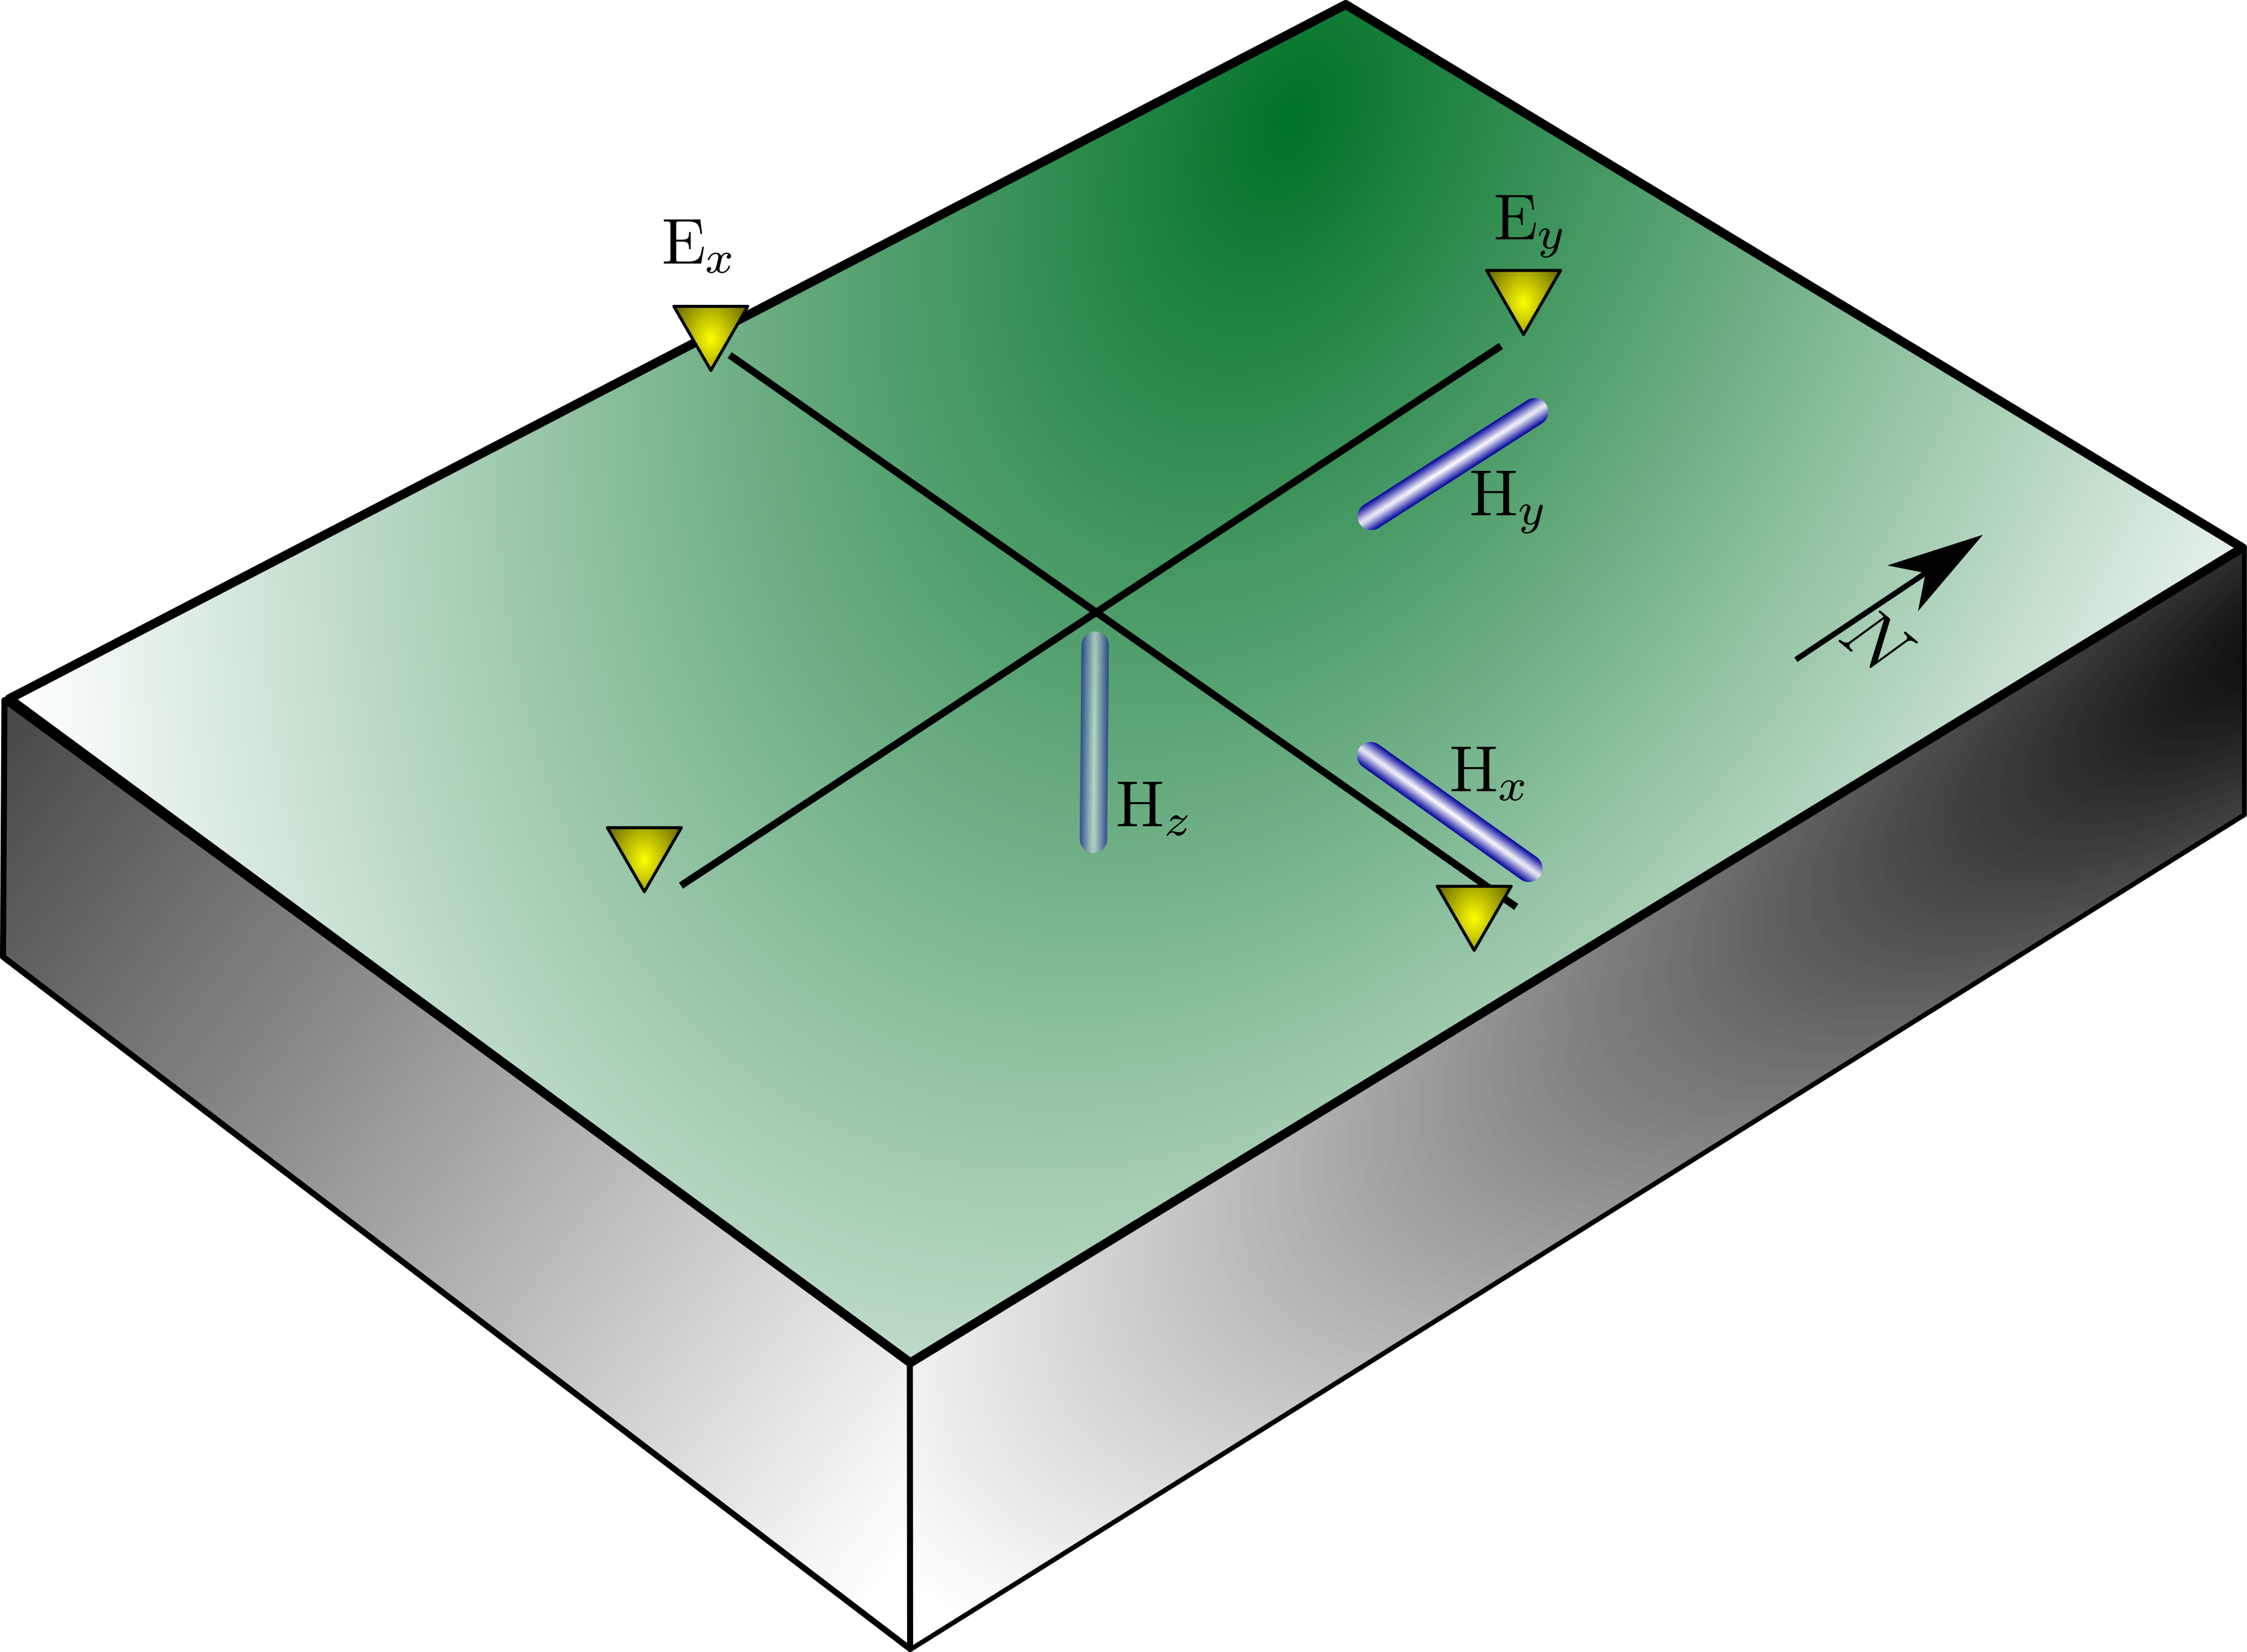
\includegraphics[width=10cm]{fig/ADU_MODELO.png}
        \end{center}
        \legend{\Fonte{\oautor}}
    \end{figure}
     O método geofísico \index{magnetotelúrico}, utiliza as baixas frequências do espectro eletromagnético, para investigar a subsuperfície do planeta Terra. A interação do vento solar com o campo magnético terrestre, compõe a origem dessas ondas eletromagnéticas.
     
     \begin{figure}[htp]
        \caption{Modelo de Aquisição para ADU}
        \begin{center}
         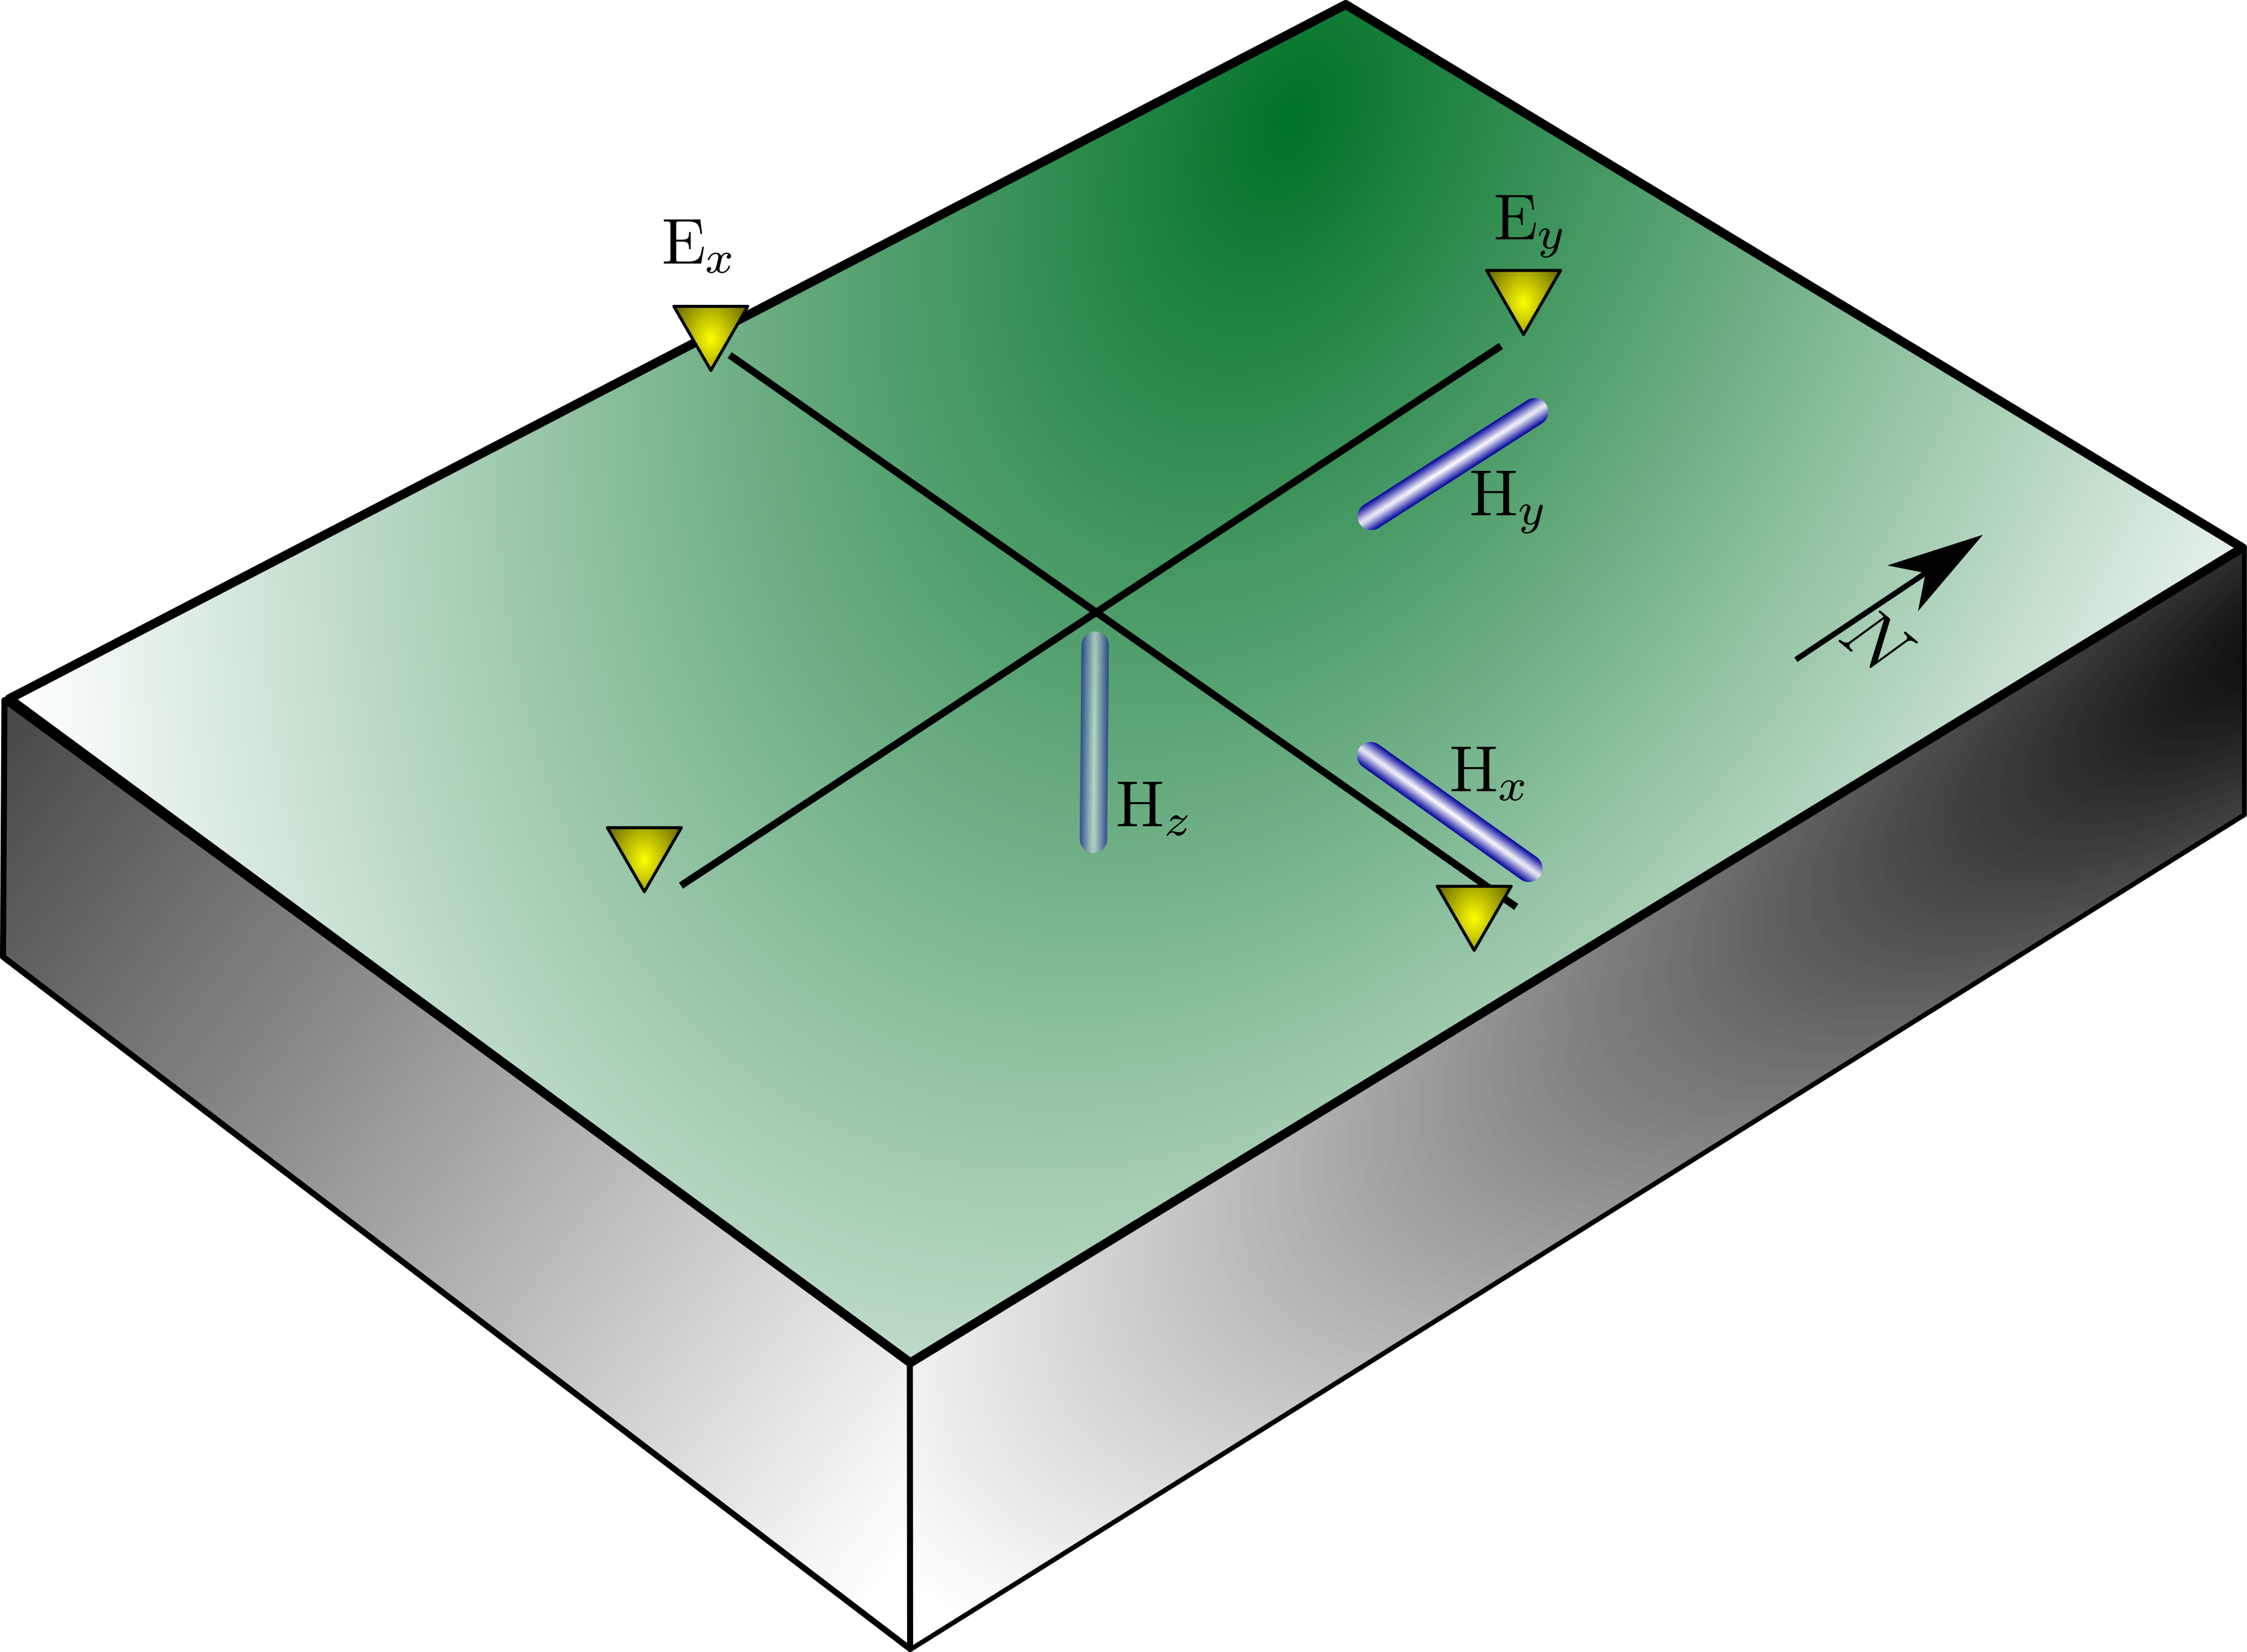
\includegraphics[width=10cm]{fig/ADU_MODELO.png}
        \end{center}
        \legend{\Fonte{\oautor}}
    \end{figure}

    \section{Uma secção}
        vamos colocar um equação beta aqui 
        
        \begin{equation}
         V = d^2
        \end{equation}
        
        vamos citar o marcelo kkkkk \cite{padua2004estudos}

    
    \subsection{Uma subsection}
    \subsubsection{UMA SUBSUSBUSBSECÇÃO}


    \chapter{EXEMPLO DE TABELA}
    
    aqui vamos colocar algumas tabelas
    
    \begin{table}[htb]
        \IBGEtab{%
            \caption{Um Exemplo de tabela alinhada conforme IBGE}%
        \label{tabela-ibge}
        }{%
            \normalsize
            \begin{tabular}[]{cp{1cm}cp{1cm}c}
             \toprule
             Nome &\qquad & Nascimento & \qquad& Documento \\
                  &            &            \\
             \midrule 
             Maria da Silva && 11/11/11 && 111.111.111 \\
             Maria da Silva && 11/11/11 && 111.111.111 \\
             Maria da Silva && 11/11/11 && 111.111.111 \\
             Maria da Silva && 11/11/11 && 111.111.111 \\
             \\
             \bottomrule
            \end{tabular}%
        }{%
            \Fonte{\oautor}%
        }
    \end{table}

    \chapter{Outro capitulo}
    
    \begin{table}[htb]
        \IBGEtab{%
            \caption{Um Exemplo de tabela alinhada conforme IBGE}%
            \label{tabela-ibge2}
        }{%
            \normalsize
            \begin{tabular}[]{cp{1cm}cp{1cm}c}
             \toprule
             Nome &\qquad & Nascimento & \qquad& Documento \\
                  &            &            \\
             \midrule 
             Maria da Silva && 11/11/11 && 111.111.111 \\
             Maria da Silva && 11/11/11 && 111.111.111 \\
             Maria da Silva && 11/11/11 && 111.111.111 \\
             Maria da Silva && 11/11/11 && 111.111.111 \\
             \\
             \bottomrule
            \end{tabular}%
        }{%
            \Fonte{\oautor}%
        }
    \end{table}
    \chapter{qualquer um}
        \index{magnetotelúrico}

% ==============================================================================

        
% PÓS-TEXTUAL
% ==============================================================================
\postextual     % Inicia os elementos pós-textuais
% ==============================================================================


% REFERENCIAS
% ==============================================================================
\bibliography{bibliografia}         % Imprime a referencia bibliografica
% ============================================================================== 
 
 
% APÊNDICE
% ==============================================================================
\apendices                      % Inicia os apêndices

\chapter{Codigo fonte}
    Conteudo do apendice A
% ==============================================================================


% ANEXO
% ==============================================================================
\anexos                         % Inicia os anexos

\chapter{Amigem para mostrar}
    Um anexo
% ==============================================================================

    
% INDICE
% ==============================================================================
% Para utilizar o indexamento automatico use no corpo do texto:
%   \index{palavra} 
%
\printindex             % Imprime o indice
% ==============================================================================

\end{document}
